\documentclass[12pt]{article}

\setlength{\parindent}{0pt}
\setcounter{secnumdepth}{3}
\usepackage[margin=1in]{geometry}

% packages
\usepackage{amsmath, amsfonts, amsthm, amssymb}
\usepackage{graphicx, float}
\usepackage{mathtools}
\usepackage{titlesec}
\usepackage{interval}
\usepackage{hyperref}
\usepackage{siunitx}
\usepackage{titling}
\usepackage{vwcol}
\usepackage{setspace}
\usepackage{empheq}
\usepackage{cancel}
\usepackage{esdiff}
\usepackage{multicol}
\usepackage{mdframed}
\usepackage{esdiff}
\usepackage{tikzsymbols}
\usepackage{multicol}
\usepackage{tikz}
\usepackage{varwidth}
\usepackage{pgfplots}
\usepackage{fancyhdr}
\usepackage{enumitem}
\usepackage{tcolorbox}

\intervalconfig {
	soft open fences
}

% header
\pagestyle{fancy}
\fancyhf{}
\lhead{Ethan Fan}
\rhead{PCH}
\cfoot{\thepage}

% section format
\titleformat{\section}
  {\bfseries}
  {}
  {0em}
  {}
\titlespacing*{\section}{0pt}{0pt}{0.3em}

\titleformat{\subsection}[runin]
  {\bfseries}
  {}
  {0em}
  {}
\titlespacing*{\subsection}{0pt}{0pt}{0em}

\titleformat{\subsubsection}[runin]
  {\itshape}
  {(\roman{subsubsection})}
  {0em}
  {}

% commands
\newcommand{\alignedintertext}[1]{%
  \noalign{%
    \vskip\belowdisplayshortskip
    \vtop{\hsize=\linewidth#1\par
    \expandafter}%
    \expandafter\prevdepth\the\prevdepth
  }%
}

\newcommand*{\paren}[1]{\ensuremath\left(#1\right)}
\newcommand*{\limit}[2][x]{\ensuremath{\displaystyle\lim_{#1\to#2}}}
\newcommand*{\Limit}[3][x]{\ensuremath{\displaystyle\lim_{#1\to#2}\left[#3\right]}}
\newcommand*{\deriv}[1][x]{\ensuremath{\dfrac{\mathrm{d}}{\mathrm{d}#1}}}
\newcommand*{\Deriv}[2][x]{\ensuremath{\dfrac{\mathrm{d}}{\mathrm{d}#1}\left[#2\right]}}
\newcommand{\dydx}{\frac{dy}{dx}}
\newcommand*{\iinteg}[2][x]{\ensuremath{\displaystyle\int #2\;\mathrm{d}#1}}
\newcommand*{\dinteg}[4][x]{\ensuremath{\displaystyle\int_{#2}^{#3}#4\;\mathrm{d}#1}}
\newcommand*{\abs}[1]{\ensuremath{\left|#1\right|}}
\newcommand*{\eps}{\varepsilon}
\newcommand*{\real}{\ensuremath\mathbb{R}}
\newcommand*{\integer}{\ensuremath\mathbb{Z}}
\newcommand*{\posint}{\ensuremath\mathbb{Z^+}}
\newcommand*{\cbrt}[1]{\ensuremath{\sqrt[3]{#1}}}
\newcommand*{\lheqzero}{\ensuremath{\underset{\text{L'H}}{\overset{\left[\frac00\right]}{=}}}}
\newcommand*{\lheqinfty}{\ensuremath{\underset{\text{L'H}}{\overset{\left[\frac{\infty}{\infty}\right]}{=}}}}
\newcommand{\tor}{\text{ or }}
\newcommand{\floor}[1]{\lfloor #1 \rfloor}

\newcommand{\vem}{\vspace{0.5em}}
\newcommand{\example}[1]{\section{Example #1}}
\newcommand{\problem}[1]{\section{Problem #1}}
\newcommand{\subproblem}[1]{\subsection{(#1)} \,}

\DeclareMathOperator{\dne}{DNE}
\DeclareMathOperator{\sgn}{sgn}

\newcommand{\definition}[1]{\begin{tcolorbox}[colback=red!5!white,colframe=red!75!black,parbox=false] #1 \end{tcolorbox}}

\newcommand{\theorem}[2]{\begin{tcolorbox}[title={#1},colback=blue!5!white,colframe=blue!75!black,parbox=false] #2 \end{tcolorbox}}

\allowdisplaybreaks
% \postdisplaypenalty=100000

% document
\begin{document}

\vspace*{0cm}

% opening
\begin{center}
    {\Large \bfseries Problem Set 69} \\[0.5cm]
    {\large How Derivatives Affect the Shape of a Graph} \\[0.35cm]
    {\normalsize April 27, 2026}
\end{center}

% problems

\problem{2}
The graph of the derivative of $f'$ of a function $f$ is shown in Figure 2. \vem

\subproblem{a}
On what intervals is $f$ increasing or decreasing?
\begin{align*}
    f'(x)>0, &\quad  \forall x\in (1,5)\\
    f'(x)<0, &\quad \forall x \in  (0,1) \cup (5,6)
\end{align*}
$f(x)$ is increasing on $(1,5)$ because $f'(x)>0$ on this interval. \vem

$f(x)$ is decreasing on $(0,1)$ and $(5,6)$ because $f'(x)>0$ on these intervals. \vem 

\subproblem{b}
At what values of $x$ does $f$ have a local maximum or minimum?
\begin{gather*}
    f'(x)=0 \implies x=1 \tor 5
\end{gather*}
$f'(x)$ changes from negative to positive at $x=1$. Therefore, $f(x)$ has a local minimum at $x=1$. \vem

$f'(x)$ changes from positive to negative at $x=5$. Therefore, $f(x)$ has a local maximum at $x=5$. \vem 

\problem{4}
Find the local maximum and minimum values of the function $g(x)=x+2 \sin x ,\  0 \le x \le 2\pi$.
\begin{gather*}
    g'(x)=2\cos x+1\\
    g'(x)=0 \implies \cos x=-\frac{1}{2}\\
    x=\frac{2\pi}{3} \tor \frac{4\pi}{3}\\
    g'(x)>0, \quad \forall x\in [0, \frac{2\pi}{3}) \cup (\frac{4\pi}{3}, 2\pi]\\
    g'(x)<0, \quad \forall x \in (\frac{2\pi}{3}, \frac{4\pi}{3})
\end{gather*}
$g'(x)$ changes from positive to negative at $x=\dfrac{2\pi}{3}$. Therefore, $g(x)$ has a local maximum at $x=\dfrac{2\pi}{3}$. \vem

$g'(x)$ changes from negative to positive at $x=\dfrac{4\pi}{3}$. Therefore, $g(x)$ has a local minimum at $x=\dfrac{4\pi}{3}$.
\begin{gather*}
    g(\frac{2\pi}{3})=\frac{2\pi}{3}+2\sin \frac{2\pi}{3}=\frac{2\pi}{3}+\sqrt{3}\\
    g(\frac{4\pi}{3})=\frac{4\pi}{3}+2\sin \frac{4\pi}{3}=\frac{4\pi}{3}-\sqrt{3}\\
    \boxed{\max: \frac{2\pi}{3}+\sqrt{3}, \min: \frac{4\pi}{3}-\sqrt{3}}
\end{gather*}

\problem{5}
Sketch a possible graph of a function $f$ that satisfies the following conditions:
\begin{enumerate}
    \item[(i)] $f'(x) > 0$ on $(-\infty, 1)$, $f'(x) < 0$ on $(1, \infty)$
    \item[(ii)] $f''(x) > 0$ on $(-\infty, -2)$ and $(2, \infty)$, $f''(x) < 0$ on $(-2, 2)$
    \item[(iii)] $\lim\limits_{x \to -\infty} f(x) = -2, \lim\limits_{x \to \infty} f(x) = 0$
\end{enumerate}
\begin{figure}[H]
    \centering
    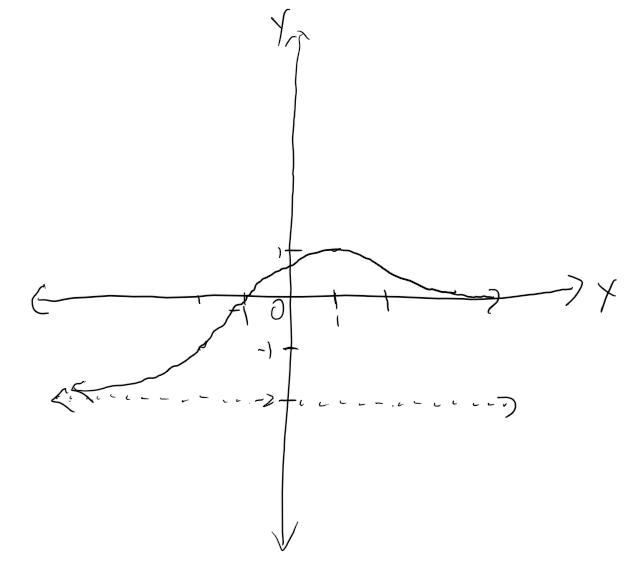
\includegraphics[width=0.5\linewidth]{q5.png}
\end{figure}

\problem{6}
For each of the functions given below:
\begin{itemize}
    \item Find the intervals on which $f$ is increasing or decreasing.
    \item Find the local maximum and minimum values of $f$.
    \item Find the intervals of concavity and the inflection points.
\end{itemize}

\subproblem{b}
$f(x)=e^{2x}+e^{-x}$
\begin{gather*}
    f'(x)=2e^{2x}-e^{-x}\\
    f'(x)=0 \implies 2e^{2x}=e^{-x}\\
    \ln 2 + 2x=-x\\
    x=-\frac{\ln 2}{3}\\
    f'(x)>0, \quad \forall x>-\frac{\ln 2}{3}\\
    f'(x)<0, \quad \forall x<-\frac{\ln 2}{3}
\end{gather*}
$f(x)$ is increasing on $(-\dfrac{\ln 2}{3}, \infty)$ because $f'(x)>0$ on this interval.

$f(x)$ is decreasing on $(-\infty , -\dfrac{\ln 2}{3})$ because $f'(x)<0$ on this interval.

$f'(x)$ changes from negative to positive at $x=-\dfrac{\ln 2}{3}$. Therefore, $f(x)$ has a local minimum at $x=-\dfrac{\ln 2}{3}$.
\begin{gather*}
    f(-\frac{\ln 2}{3})=e^{-\frac{2\ln 2}{3}}+e^{\frac{\ln 2}{3}}=\frac{1}{\cbrt{4}}+\cbrt{2}\\
    \boxed{\min : \frac{1}{\cbrt{4}}+\cbrt{2}}\\
    f''(x)=4e^{2x}+e^{-x}\\
    f''(x)>0
\end{gather*}
$f(x)$ is concave up on $\mathbb{R}$ because $f''(x)>0$ on $\mathbb{R}$. \vem

There are no inflection points.  \vem 

\subproblem{c}
$f(x)=\dfrac{\ln x}{\sqrt{x}}$
\begin{gather*}
    x>0\\
    f'(x)=\frac{\frac{\sqrt{x}}{x}-\frac{\ln x}{2\sqrt{x}}}{x}=\frac{2-\ln x}{2x\sqrt{x}}\\
    f'(x)=0\implies \ln x=2\implies x=e^2\\
    f'(x)>0, \quad \forall 0<x <e^2\\
    f'(x)<0, \quad \forall x >e^2
\end{gather*}
$f(x)$ is increasing on $(0, e^2)$ because $f'(x)>0$ on this interval.\vem

$f(x)$ is decreasing on $(e^2, \infty)$ because $f'(x)<0$ on this interval. \vem

$f'(x)$ changes from positive to negative at $x=e^2$. Therefore, $f(x)$ has a local maximum at $x=e^2$.
\begin{gather*}
    f(e^2)=\frac{\ln e^2}{\sqrt{e^2}}=\frac{2}{e}\\
    \boxed{\max: \frac{2}{e}}\\
    f''(x)=\frac{(\ln x-2)3\sqrt{x}-2\sqrt{x}}{4x^3}\\
    f''(x)=0 \implies 3\ln x = 8 \implies x= e^{\frac{8}{3}}\\
    f''(x)>0, \quad \forall x > e^{\frac{8}{3}}\\
    f''(x)<0, \quad \forall 0 <x < e^{\frac{8}{3}}
\end{gather*}
$f(x)$ is concave up on $(e^{\frac{8}{3}}, \infty)$ because $f''(x)>0$ on this interval. \vem

$f(x)$ is concave down on $(0, e^{\frac{8}{3}})$ because $f''(x)<0$ on this interval. \vem

Inflection point: $\boxed{x=e^{\frac{8}{3}}}$ \vem

\problem{7}
Find the local maximum and minimum values of $f$ using both the First and Second Derivative Tests. Which methods do you prefer? \vem 

\subproblem{a}
$f(x)=x^5-5x+3$
\begin{gather*}
    f'(x)=5x^4-5\\
    f'(x)=0 \implies x^4=1 \implies x=1 \tor -1\\
    f'(x)>0, \quad x\in (-\infty ,-1) \cup (1,\infty)\\
    f'(x)<0, \quad x\in (-1,1)
\end{gather*}
$f'(x)$ changes from positive to negative at $x=-1$. Therefore, $f(x)$ has a local maximum at $x=-1$. \vem

$f'(x)$ changes from negative to positive at $x=1$. Therefore, $f(x)$ has a local minimum at $x=1$. 
\begin{gather*}
    f''(x)=20x^3\\
    f''(1)>0, f''(-1)<0
\end{gather*}
$f'(1)=0$ and $f''(1)>0$. Therefore, $f(x)$ has a local minimum at $x=1$.\vem

$f'(-1)=0$ and $f''(-1)<0$. Therefore, $f(x)$ has a local maximum at $x=-1$. 
\begin{gather*}
    f(1)=1^5-5\cdot1+3=-1\\
    f(-1)=(-1)^5-5\cdot (-1)+3=7\\
    \boxed{\max:7, \min :-1}
\end{gather*}

\subproblem{b}
$f(x)=x+\sqrt{1-x}$
\begin{gather*}
    x<1\\
    f'(x)=1-\frac{1}{2\sqrt{1-x}}\\
    f'(x)=0 \implies 1=2\sqrt{1-x}\\
    x=\frac{3}{4} \tor 1\\
    f'(x)>0, \quad x<\frac{3}{4}\\
    f'(x)<0, \quad \frac{3}{4}<x<1
\end{gather*}
$f'(x)$ changes from positive to negative at $x=\dfrac{3}{4}$. Therefore, $f(x)$ has a local maximum at $x=\dfrac{3}{4}$.
\begin{gather*}
    f''(x)=-\frac{1}{4(1-x)^{\frac{3}{2}}}\\
    f''(x)<0
\end{gather*}
$f'(\dfrac{3}{4})=0$ and $f''(\dfrac{3}{4})<0$. Therefore, $f(x)$ has a local maximum at $x=\dfrac{3}{4}$.
\begin{gather*}
    f(\frac{3}{4})=\frac{3}{4}+\sqrt{1-\frac{3}{4}}=\frac{5}{4}\\
    \boxed{\max:\frac{5}{4}}
\end{gather*}

\problem{8}
The graph of the derivative $f'$ of a continuous function $f$ is shown in Figure 4. \vem

\subproblem{a}
On what intervals is $f$ increasing or decreasing?
\begin{align*}
    f'(x)>0,&\quad \forall x \in (3,6) \cup (6,9)\\
    f'(x)<0,&\quad \forall x \in (0,3)
\end{align*}
$f(x)$ is increasing on $(3,6) \cup (6,9)$ because $f'(x)>0$ on this interval. \vem

$f(x)$ is decreasing on $(0,3)$ because $f'(x)<0$ on this interval. \vem

\subproblem{b}
At what values of $x$ does $f$ have a local maximum or minimum? \vem

$f'(x)$ changes from negative to positive at $x=4$ and $x=8$. Therefore, $f(x)$ has local minimums at $x=4$ and $x=8$. \vem

$f'(x)$ changes from positive to negative at $x=2$. Therefore, $f(x)$ has a local maximum at $x=2$. \vem 

\subproblem{c}
On what intervals is $f$ concave upward or downward?
\begin{align*}
    f''(x)>0, &\quad \forall x \in (3,6) \cup (6,9)\\
    f''(x)<0, &\quad \forall x \in (0,3)
\end{align*}
$f(x)$ is concave upward on $(3,6)$ and $(6,9)$ because $f''(x)>0$ on these intervals. \vem

$f(x)$ is concave downward on $(0,3)$ because $f''(x)<0$ on this interval. \vem

\subproblem{d}
State the $x$-coordinate(s) of the point(s) of inflection. \vem

$f(x)$ changes from concave downward to concave upward at $x=3$. Therefore, $x=3$ is an inflection point. \vem

\subproblem{e}
\begin{figure}[H]
    \centering
    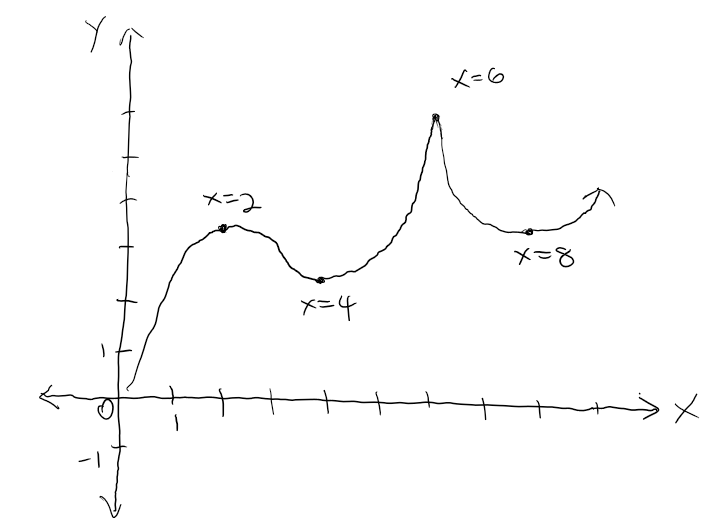
\includegraphics[width=0.5\linewidth]{q8.png}
\end{figure}

\problem{9}
Suppose $f''$ is continuous on $(-\infty, \infty)$. \vem

\subproblem{a}
If $f'(2) = 0$ and $f''(2) = -5$, what can you say about $f$? \vem

$f(x)$ has a local maximum at $x=2$. \vem

\subproblem{b}
If $f'(6) = 0$ and $f''(6) = 0$, what can you say about $f$? \vem

$f(x)$ has a local maximum, local minimum, or neither at $x=6$. \vem

\problem{11}
Suppose the derivative of a function $f$ is $f'(x) = (x+1)^2(x-3)^5(x-6)^4$. On what interval is $f$ increasing?
\begin{gather*}
    f'(x) = (x+1)^2(x-3)^5(x-6)^4\\
    f'(x)=0 \implies x=-1,3,6\\
    f'(x)>0, \quad \forall x \in (3,6) \cup (6,\infty)\\
    f'(x)<0, \forall x \in (-\infty,-1) \cup (-1,3)
\end{gather*}
$f(x)$ is increasing on $(3,6)$ and $(6,\infty)$ as $f'(x)>0$ on these intervals. \vem

\problem{12}
Let $K(t)$ be a measure of the knowledge you gain by studying for a test for $t$ hours. Which do you think is larger, $K(8) - K(7)$ or $K(3) - K(2)$? Is the graph of $K$ concave upward or concave downward? Why?
\vem

Given the knowledge gained per hour decreases with time. By inspection, we define $K(t)$ as $\ln x$.
\begin{gather*}
    K'(t)=\frac{1}{x}\\
    K''(t)=-\frac{2}{x^2}\\
    \boxed{K(3)-K(2)>K(8)-K(7)}
\end{gather*}
$K(t)$ is concave downward because $K''(t)<0$. \vem

\problem{13}
Find a cubic function $f(x) = ax^3 + bx^2 + cx + d$ that has a local maximum value of $3$ at $x = -2$ and a local minimum value of $0$ at $x = 1$.
\[
f'(x)=3ax^2+2bx+c
\] 
\vspace{-2.5em}
\begin{align}
    f(-2)&=-8a+4b-2c+d=3\\
    f(1)&=a+b+c+d=0\\
    f'(-2)&=12a-4b+c=0\\
    f'(1)&=3a+2b+c=0
\end{align}
 \vspace{-2.5em}
\begin{gather*}
    (2)-(1) \implies 3a-b+c=-1\\
    (4)-(2)+(1) \implies 3b=1 \implies b=\frac{1}{3}\\
    (4)-(3) \implies 2b=3a \implies a=\frac{2}{9}\\
    c=-\frac{4}{3},d=\frac{7}{9}\\
    \boxed{f(x)=\frac{2}{9}x^3+\frac{1}{3}x^2-\frac{4}{3}x+\frac{7}{9}}
\end{gather*}

\problem{14}
Show that the curve $\displaystyle y = \frac{1+x}{1+x^2}$ has three points of inflection and they all lie on one straight line.
\begin{align*}
    f'(x)=&\frac{(1+x^2)-2x(1+x)}{(1+x^2)^2}=\frac{-x^2-2x+1}{(1+x^2)^2}\\
    f''(x)=&\frac{(1+x^2)^2(-2x-2)-4x(-x^2-2x+1)(1+x^2)}{(1+x^2)^4}\\
    =&\frac{(1+x^2)(-2x^3-2x^2-2x-2+4x^3+8x^2-4x)}{(1+x^2)^4}\\
    =&\frac{(1+x^2)(2x^3+6x^2-6x-2)}{(1+x^2)^4}\\
    f''(x)=&0 \implies x^3+3x^2-3x-1=0
\end{align*}
\vspace{-2.5em}
\begin{gather*}
    x=1 \implies (x-1)(x^2+4x+1)=0\\
    x=\frac{-4\pm2\sqrt{3}}{2}\\
    \boxed{x=1,-2\pm \sqrt{3}}\\
    \begin{cases}
        f(1)=1\\
    f(-2+\sqrt{3})=\dfrac{\sqrt{3}+1}{4}\\
    f(-2-\sqrt{3})=\dfrac{1-\sqrt{3}}{4}
    \end{cases}\\
    \dydx=\frac{f(1)-f(-2+\sqrt{3})}{1-(-2+\sqrt{3})}=\frac{\frac{3-\sqrt{3}}{4}}{3-\sqrt{3}}=\frac{1}{4}\\
    \dydx=\frac{f(1)-f(-2-\sqrt{3})}{1-(-2-\sqrt{3})}=\frac{\frac{3+\sqrt{3}}{4}}{3+\sqrt{3}}=\frac{1}{4}\\
    \boxed{\text{Three points of inflection are collinear}}
\end{gather*}

\problem{15}
Suppose $f$ is differentiable on an interval $I$ and $f'(x) > 0$ for all numbers $x$ in $I$ except for a single number $c$. Prove that $f$ is increasing on the entire interval $I$. \vem

Given $f(x)$ is increasing on an interval $I$ except for a single value $c$, as $f'(x)>0$ on these intervals, let $x_1,x_2$ be arbitrary values on $I$ s.t. $x_1<x_2$. \vem

For $x_1<x_2 \le c$, as $f(x)$ is increasing on $(x_1,c)$, $f(x_1)<f(x_2)$. \vem

For $c \le x_1<x_2$, as $f(x)$ is increasing on $(c,x_2)$, $f(x_1)<f(x_2)$.\vem

For $x_1 < c< x_2$, as $f(x)$ is increasing on $(x_1,c)$ and $(c,x_2)$, then $f(x_1)<f(c)$ and $f(c)<f(x_2)$. Thus, $f(x_1)<f(x_2)$.\vem

Therefore, $f(x_1)<f(x_2)$ for all $x_1<x_2$ on $I$.

\end{document}

